\section{76 - MAT - AG 2.1, AN 1.3, AN 3.2, AN 3.3, AN 4.2, FA 1.4, FA 1.7, FA 2.6, WS 1.3 - Laufband - BIFIE Aufgabensammlung}

\begin{langesbeispiel} \item[0] %PUNKTE DES BEISPIELS
	
Ein Laufband ist ein Sportgerät, auf dem verschiedene Lauftrainingsprogramme absolviert werden können.

Bei einem individuell erstellen, 30-minütigen Trainingsprogramm ändert sich die Laufbahngeschwindigkeit alle zwei Minuten. Die von der Zeit $t$ (in min) abhängigen Laufbahngeschwindigkeiten (in km/h) sind Funktionswerte an bestimmten Stellen der Funktion $f$ mit $f(t)=0,0008\cdot t³-0,05\cdot t²+1,1\cdot t+5$.

Die Laufbahngeschwindigkeit während der ersten beiden Minuten entspricht dem Funktionswert $f(0)$, die Geschwindigkeit in den beiden darauffolgenden Minuten dem Wert $f(2)$ usw. Für die Berechnung wird vereinfacht angenommen, dass sich die Laufbandgeschwindigkeit innerhalb sehr kurzer Zeit ändert.

Die nachstehende Abbildung zeigt modellhaft die Entwicklung der Laufbahngeschwindigkeit in den ersten zehn Minuten des Trainings, wobei $v(t)$ die Geschwindigkeit des Laufbands zum Zeitpunkt $t$ angibt. Das Training beginnt zum Zeitpunkt $t=0$.

\begin{center}
	\resizebox{0.7\linewidth}{!}{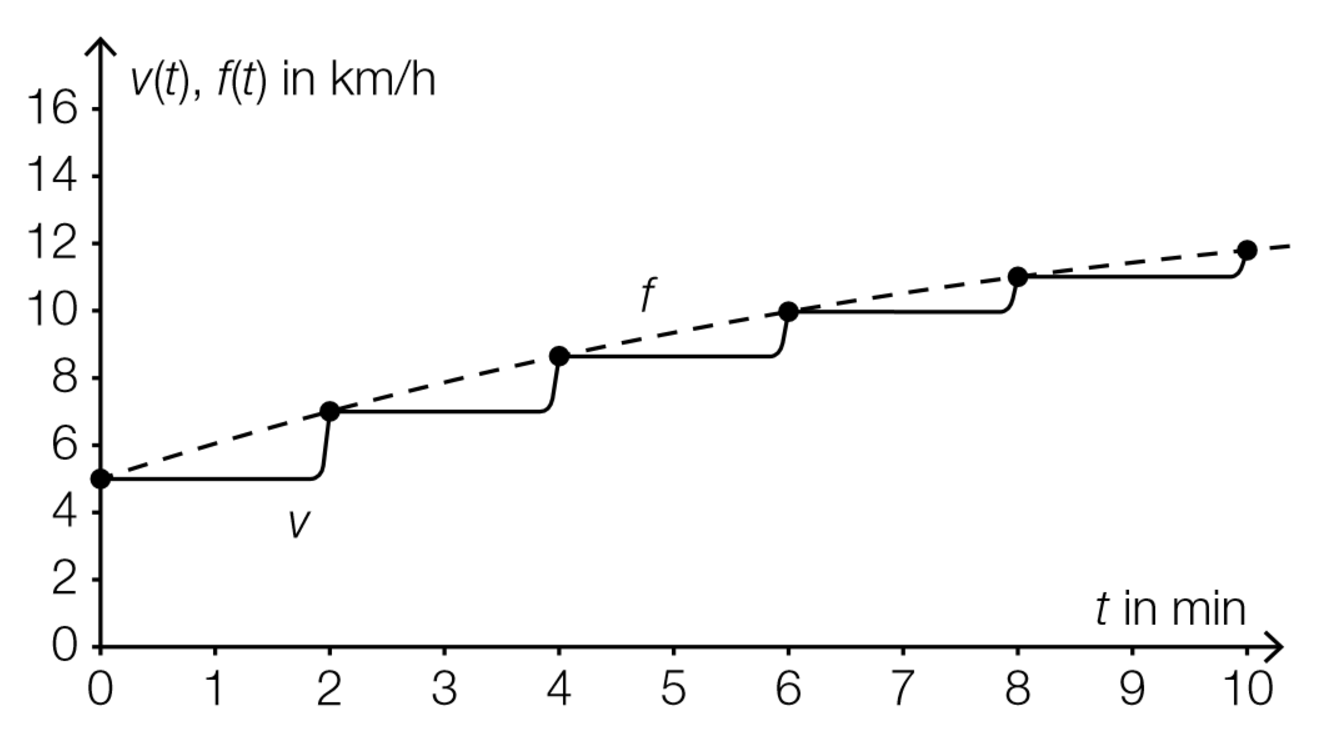
\includegraphics{../Bilder/Bild76-1.eps}}
\end{center}

\subsection{Aufgabenstellung:}
\begin{enumerate}
	\item Gib einen Ausdruck an, mit dem das arithmetische Mittel der Laufbandgeschwindigkeiten während des 30-minütigen Trainingsprogramms berechnet werden kann, und ermittle diesen Wert!\leer
	
	Begründe, warum das arithmetische Mittel der Laufbandgeschwindigkeiten der mittleren Geschwindigkeit $\bar{v}$ während des 30-minütigen Trainingsprogramms entspricht!
	
	Berechne unter Verwendung der mittleren Geschwindigkeit $\bar{v}$ die während des 30-minütigen Trainingsprogramms bewältigte Strecke!
	
	\item Gib die minimale und die maximale Geschwindigkeit des Laufbands während des 30-minütigen Trainingsprogramms an!\leer
	
	$v_\text{min}=$ \rule{5cm}{0.3pt}\,km/h\leer
	
	$v_\text{max}=$ \rule{5cm}{0.3pt}\,km/h\leer
	
	Begründe, warum zu den Zeitpunkten $t_{\text{min}}$ und $t_{\text{max}}$, zu denen die minimale bzw. die maximale Geschwindigkeit des Laufbands in dem 30-minptigen Trainingsprogramm erreicht wird, $f'(t_{\text{min}})\neq 0$ und $f'(t_\text{max})\neq 0$ gilt!\leer
	
	\item Gib den Wert von $v'(1)$ an und interpretiere diesen Wert (mit Angabe der Einheit) im gegebenen Kontext!\leer
	
	$v'(1)=$ \rule{5cm}{0.3pt}\leer
	
	Beschreibe anhand des Graphen in der Einleitung, wie der Graph der Ableitungsfunktion $v'$ im Intervall $[0;30]$ verlaufen müsste!\leer
	
	\item Die in den ersten zehn Trainingsminuten zurückgelegte Weglänge kann näherungsweise mit dem Integral $\frac{1}{60}\cdot\int^{10}_0{f(t)}$d$t$ berechnet werden.
	
	Berechne diesen Näherungswert und erläuter die Bedeutung des Faktors $\frac{1}{60}$!\leer
	
	Gib die absolute Abweichung des berechneten Näherungswertes von der tatsächlich zurückgelegten Weglänge während der ersten zehn Minuten in Metern an!	\leer
	
	\item Unter bestimmten Voraussetzungen ist der Energiebedarf einer Person bei einem Lauftraining direkt proportional zur Masse der Person (in kg) und zur zurückgelegten Weglänge (in km).

Die nachstehende Tabelle zeigt den Energiebedarf (in kcal) einer 80\,kg schweren Person bei einem Lauftraining in Abhängigkeit von der Dauer $t$ des Trainings. Die Person läuft mit einer konstanten Geschwindigkeit von 10\,km/h.

\begin{center}
	\begin{tabular}{|l|l|l|l|l|}\cline{2-5}
	\multicolumn{1}{c|}{}&$t=15$\,min&$t=30$\,min&$t=45$\,min&$t=60$\,min\\ \hline
	Energiebedarf in kcal&194&388&582&776\\ \hline	
	\end{tabular}
\end{center}

Zeige anhand der Tabellenwerte die direkte Proportionalität des Energiebedarfs zur zurückgelegten Wegstrecke und berechne den Proportionalitätsfaktor $k$!

Beim Lauftraining wird die Geschwindigkeit häufig als "`Tempo"' in min/km umschrieben. Berechne für die unten angeführten Geschwindigkeiten unter Verwendung des Proportionalitätsfaktors $k$ für eine 90\,kg schwere Person jeweils das Tempo und den Energiebedarf (in kcal) für die angegebene Zeitdauer!

\begin{center}
	\begin{tabular}{|p{3cm}|p{3cm}|p{3cm}|p{3cm}|}\hline
	\multirow{2}{2cm}{Geschwindigkeit in km/h}&\multirow{2}{2cm}{Tempo in min/km}&\multirow{2}{2cm}{Energiebedarf in 15\,min}&\multirow{2}{2cm}{Energiebedarf in 30\,min}\\
	&&&\\ \hline \hline
	\multicolumn{1}{|c|}{7,5}&\multicolumn{1}{c|}{8}&&\\ \hline
	\multicolumn{1}{|c|}{10}&&&\\ \hline
	\multicolumn{1}{|c|}{12}&&&\\ \hline	
	\end{tabular}
\end{center}
\end{enumerate}

\antwort{
\begin{enumerate}
	\item \subsection{Lösungserwartung:} 

$\bar{v}=\frac{1}{15}\cdot(f(0)+f(2)+f(4)+...+f(28)\approx 11,57$

Das arithmetische Mittel der Laufbahngeschwindigkeiten beträgt 11,57\,km/h\leer

Das Arithmetische Mittel entspricht der mittleren Geschwindigkeit während des 30-minütigen Trainingsprogramms, weil die Geschwindigkeiten $v(0),...,v(28)$ in gleich langen Zeitintervallen (2\,min) jeweils konstant sind.\leer

zurückgelegte Weglänge: $0,5\,\text{h}\cdot 11,57\,\text{km/h}=5,785$\,km

	\item \subsection{Lösungserwartung:}
	
	$v_\text{min}=5$\,km/h
	
	$v_\text{max}=14,16$\,km/h\leer
	
	$t_\text{min}$ und $t_\text{max}$ sind keine lokalen Extremstellen der Funktion $f$, weshalb die 1. Ableitung von $f$ an diesen Stellen nicht null ist.

\item \subsection{Lösungserwartung:}
	
$v'(1)=0$

Mögliche Interpretationen:

Die Beschleunigung (momentane Geschwindigkeitsänderung) des Laufbands nach 1 Minute beträgt 0\,m/s$²$.

oder:

Das Laufband (die Läuferin/der Läufer) bewegt sich während der ersten 2 Minuten mit konstanter Geschwindigkeit, d.h., seine Beschleunigung ist zum Zeitpunkt $t=1$\,min gleich null.\leer

Der Graph von $v'$ würde auf der 1. Achse verlaufen und nur zu den Zeitpunkten der Geschwindigkeitsänderungen $(t=2, t=4, t=6,...)$ sehr hohe Werte annehmen.

\item \subsection{Lösungserwartung:}
	
$\frac{1}{60}\cdot\int^{10}_0{f(t)}$d$t\approx 1,506$

zurückgelegte Weglänge: ca. 1,51\,km\leer

Mögliche Begründungen:

Der Faktor $\frac{1}{60}$ ist erforderlich, um die Geschwindigkeiten von km/h in km/min umzurechnen, da die Zeiten (Intervallgrenzen) in Minuten gegeben sind (1\,h=60\,min).

oder:

Der Faktor $\frac{1}{60}$ ist erforderlich, um die pro Stunde zurückgelegten Wegstrecken auf die pro Minute zurückgelegten Wegstrecken umzurechnen.\leer

Für die tatsächlich zurückgelegte Weglänge gilt:

$\frac{2}{60}\cdot(f(0)+f(2)+f(4)+f(6)+f(8))\approx 1,388$\,km

$\Rightarrow$ Der Näherungswert für die Weglänge weicht um ca. 118\,m vom exakten Wert ab.

\item \subsection{Lösungserwartung:}
	
$194=k\cdot 80\cdot 2,5$

$k=0,97$\leer

Bei der doppelten/dreifachen/vierfachen Laufzeit wird die doppelte/dreifache/vierfache Strecke zurückgelegt und auch der Energiebedarf ist doppelt/dreimal/viermal so groß.

\begin{center}
	\begin{tabular}{|p{3cm}|p{3cm}|p{3cm}|p{3cm}|}\hline
	\multirow{2}{2cm}{Geschwindigkeit in km/h}&\multirow{2}{2cm}{Tempo in min/km}&\multirow{2}{2cm}{Energiebedarf in 15\,min}&\multirow{2}{2cm}{Energiebedarf in 30\,min}\\
	&&&\\ \hline \hline
	\multicolumn{1}{|c|}{7,5}&\multicolumn{1}{c|}{8}&\cellcolor[gray]{0.7}163,7&\cellcolor[gray]{0.7}327,4\\ \hline
	\multicolumn{1}{|c|}{10}&\cellcolor[gray]{0.7}6&\cellcolor[gray]{0.7}218,25&\cellcolor[gray]{0.7}436,5\\ \hline
	\multicolumn{1}{|c|}{12}&\cellcolor[gray]{0.7}5&\cellcolor[gray]{0.7}261,9&\cellcolor[gray]{0.7}523,8\\ \hline	
	\end{tabular}
\end{center}

\end{enumerate}}
		\end{langesbeispiel}